\documentclass[a4paper, 12pt, oneside]{article}

\usepackage[utf8]{inputenc}
\usepackage[T1]{fontenc}
\usepackage[french]{babel}
\usepackage{array}
\usepackage{shortvrb}
\usepackage{listings}
\usepackage[fleqn]{amsmath}
\usepackage{amsfonts}
\usepackage{fullpage}
\usepackage{enumerate}
\usepackage{graphicx}
\usepackage{subfigure}
\usepackage{alltt}
\usepackage{url}
\usepackage{indentfirst}
\usepackage{eurosym}
\usepackage{listings}
\usepackage{titlesec, blindtext, color}
\usepackage[table,xcdraw,dvipsnames]{xcolor}
\usepackage[unicode]{hyperref}
\usepackage{url}
\usepackage{float}

\definecolor{mygray}{rgb}{0.5,0.5,0.5}

\lstset{
    language=C, % Utilisation du langage C
    commentstyle={\color{MidnightBlue}}, % Couleur des commentaires
    frame=single, % Entoure le code d'un joli cadre
    rulecolor=\color{black}, % Couleur de la ligne qui forme le cadre
    stringstyle=\color{RawSienna}, % Couleur des chaines de caractères
    numbers=left, % Ajoute une numérotation des lignes à gauche
    numbersep=5pt, % Distance entre les numérots de lignes et le code
    numberstyle=\tiny\color{mygray}, % Couleur des numéros de lignes
    basicstyle=\tt\footnotesize, 
    tabsize=3, % Largeur des tabulations par défaut
    keywordstyle=\tt\bf\footnotesize\color{Sepia}, % Style des mots-clés
    extendedchars=true, 
    captionpos=b, % sets the caption-position to bottom
    texcl=true, % Commentaires sur une ligne interprétés en Latex
    showstringspaces=false, % Ne montre pas les espace dans les chaines de caractères
    escapeinside={(>}{<)}, % Permet de mettre du latex entre des <( et )>.
    inputencoding=utf8,
    literate=
  {á}{{\'a}}1 {é}{{\'e}}1 {í}{{\'i}}1 {ó}{{\'o}}1 {ú}{{\'u}}1
  {Á}{{\'A}}1 {É}{{\'E}}1 {Í}{{\'I}}1 {Ó}{{\'O}}1 {Ú}{{\'U}}1
  {à}{{\`a}}1 {è}{{\`e}}1 {ì}{{\`i}}1 {ò}{{\`o}}1 {ù}{{\`u}}1
  {À}{{\`A}}1 {È}{{\`E}}1 {Ì}{{\`I}}1 {Ò}{{\`O}}1 {Ù}{{\`U}}1
  {ä}{{\"a}}1 {ë}{{\"e}}1 {ï}{{\"i}}1 {ö}{{\"o}}1 {ü}{{\"u}}1
  {Ä}{{\"A}}1 {Ë}{{\"E}}1 {Ï}{{\"I}}1 {Ö}{{\"O}}1 {Ü}{{\"U}}1
  {â}{{\^a}}1 {ê}{{\^e}}1 {î}{{\^i}}1 {ô}{{\^o}}1 {û}{{\^u}}1
  {Â}{{\^A}}1 {Ê}{{\^E}}1 {Î}{{\^I}}1 {Ô}{{\^O}}1 {Û}{{\^U}}1
  {œ}{{\oe}}1 {Œ}{{\OE}}1 {æ}{{\ae}}1 {Æ}{{\AE}}1 {ß}{{\ss}}1
  {ű}{{\H{u}}}1 {Ű}{{\H{U}}}1 {ő}{{\H{o}}}1 {Ő}{{\H{O}}}1
  {ç}{{\c c}}1 {Ç}{{\c C}}1 {ø}{{\o}}1 {å}{{\r a}}1 {Å}{{\r A}}1
  {€}{{\euro}}1 {£}{{\pounds}}1 {«}{{\guillemotleft}}1
  {»}{{\guillemotright}}1 {ñ}{{\~n}}1 {Ñ}{{\~N}}1 {¿}{{?`}}1
}

%%%% Page de garde %%%%

\title{\textbf{Introduction aux processus stochastiques}\\
	   Projet 1 : Analyse de propagation d'un virus dans un réseau}
\author{Maxime GOFFART \\180521 \and Olivier JORIS\\182113}
\date{Année académique 2019 - 2020}

\begin{document}

\maketitle
\newpage

\tableofcontents
\newpage

\section{Introduction}

Les processus stochastiques permettent d'étudier des phénomènes aléatoires dans divers secteurs : l'économie, la climatologie, la météorologie, la biologie, \dotso

En particulier dans ce projet, il nous a été demandé d'étudier un phénomène d'actualité : la propagation d'un virus au sein d'un réseau, pouvant peut être modélisé à l'aide d'une chaîne de Markov. Ainsi, ce projet nous a permis d'appliquer les concepts vus au cours sur un exemple concret et d'actualité.

\section{Structure du programme} % je ne sais pas si on la met maintenant ou après, j'attends qu'on ait la structure finale du programme pour la faire

\section{Etude du modèle exact}

\subsection{Question 1}
	
	Le modèle proposé dans l'énoncé est bien un processus de Markov en temps discret caractérisé par ses $3^N$ états \footnote{$N$ étant la taille de la population.}. Les états de cette chaînes sont caractérisés par la suite de longueur $N$ des catégories \footnote{S, R ou I.} auxquelles appartiennent les individus \footnote{Les individus étant indexés de 1 à N.} à l'instant t. Par exemple : pour $N = 3$, l'état "'S' 'I' 'I'" représente le fait que le premier individu est susceptible d'être infecté et que les deux derniers sont infectés.
	
	 Les probabilités de transitions d'un état à un potentiel état de l'instant suivant de la chaîne dépendent à la fois de chacune des catégories des individus à l'instant initial et de leurs interactions avec des personnes infectées \footnote{Modélisées par le graphe $W$.}.
	
	Les états de cette chaîne qui sont uniquement composés d'individus de la catégorie 'R' ou\footnote{Il s'agit d'un "ou" inclusif.} de la catégorie 'S' sont absorbants car la propagation du virus n'est plus possible s'il n'y a plus d'infectés. Il en va de même pour les états dans lesquels les infectés n'ont de contact avec personne\footnote{Cela correspond à une ligne remplie de 0 dans le graphe $W$.}. Cette chaîne n'est donc ni irréductible, ni régulière, ni périodique.

\subsection{Question 2}

Il faudra en moyenne ... à un individu pour guérir une fois infecté.

\subsection{Question 3}

Pour répondre à cette question, le programme peut-être lancé à l'aide de la commande suivante :

\begin{lstlisting}[language=bash]
$ python3 exact_model.py matrixSize fileName wType 
\end{lstlisting}

où la première option spécifie la taille de la matrice $W$ utilisée, la deuxième représente le nom du fichier dans lequel cette matrice est encodée et la troisième permettant d'ajuster l'échelle du graphique en spécifiant si on a choisit une matrice $W_{big}$ ou $W_{lin}$\footnote{A l'aide du mot-clé "lin" ou "full"}. Ensuite, le programme demande à l'utilisateur sur combien de simulations celui-ci veut que les calculs soient effectués.\\

Ainsi, en lançant le programme avec cette commande :

\begin{lstlisting}[language=bash]
$ python3 exact_model.py 6 6x6_lin.txt lin
\end{lstlisting}

On obtient ce graphique répondant à la première partie de la question avec les paramètres $\mu$ et $\beta$ fixés aux valeurs suggérées : 

\begin{figure}[H]
	\centering
	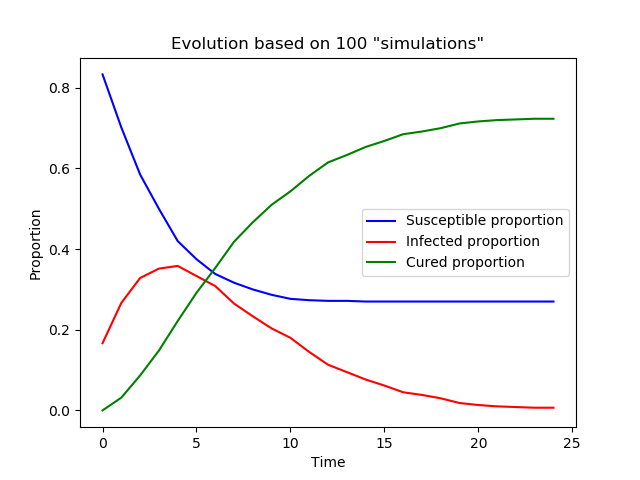
\includegraphics[scale=1]{lin_6x6.png} 
	\caption{Evolution des proportions d'individus dans chacune des catégorie au cours du temps suivant un modèle représenté par une matrice $W_{lin}$.}
\end{figure}

Sur la figure 1, on observe le fait que la proportion d'individus infectés ne cesse de diminuer. En effet, les individus ayant peu de contacts les uns avec les autres, la probabilité qu'un individu soit infecté tend vers 0. De plus, les individus infectés initialement finissent par guérir.\\

De la même façon en lançant le programme à l'aide de cette commande :

\begin{lstlisting}[language=bash]
$ python3 exact_model.py 6 6x6_full.txt full
\end{lstlisting}

On obtient ce graphique répondant à la deuxième partie de la question avec les paramètres $\mu$ et $\beta$ fixés aux valeurs suggérées : 

\begin{figure}[H]
	\centering
	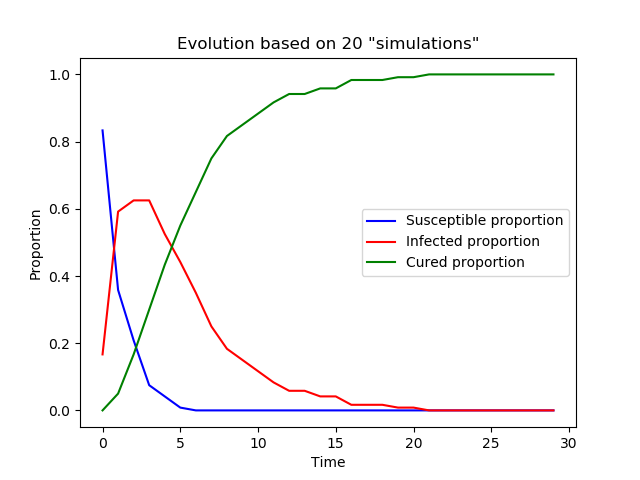
\includegraphics[scale=1]{full_6x6.png} 
	\caption{Evolution des proportions d'individus dans chacune des catégorie au cours du temps suivant un modèle représenté par une matrice $W_{full}$.}
\end{figure}

Sur la figure 2, on observe, à l'inverse de la situation précédente, que la population connaît un nombre important d'infectés. Au temps t = 25, on peut voir que la proportion d'individus susceptibles est proche de 0, c'est-à-dire que toute la population a été infecté. En effet, les individus ayant tous des contacts les uns avec les autres, le virus ne fait que se propager au sein de la population jusqu'à ce que celle-ci soit entièrement guérie.

\subsection{Question 4}


	
\end{document}